%!TEX root = vorlage.tex
% Marvin Teichmann and Martin Thoma
\section{Introduction}\label{sec:introduction}

This Tutoial aimes to give a comprehensive introduction to neuronal network based semantic segmentation. It is directed to an audients, who is already familier with semantic segmentation using traditional shallow learning methods but not with the novel deep learning approaches. The work is specied with examples and framed around applications of the field medical informatics, however the presented theory generalizes easily to other fields. 

Deep Neuronal Networks and in particular \glspl{CNN} have been the driving factor of innovation in Computer Vision in the past years. Since Krizhevsky et. al \cite{AlexNet} proposed a novel and award winning Network architecture, Deep \glspl{CNN} have broken new records in many Computer Vision Domains including Classification \cite{AlexNet,VGG16,googLeNeT}, Localization and Detection \cite{RNN,overfeat} and Semantic Segmentation tasks \cite{fcn,CRF1,googleSeg}. 

Especially Semantic Segmentation does have several interesting applications in medical informatics, including ... . A recent survey of the traditionally used methods in this area are published in \cite{Martin}. Considering the very recent break-throughs in semantic segmentation using deep learning models \cite{fcn,CRF1}, the next logical step is to adapt such models to medical informatics tasks. This paper aims to help researchers in the field of medical informatics to do so. 

\iffalse

To archive that we will give a comprehensive introduction to neuronal network based semantic segmentation. As neuronal network based semantic segmentation is a very new method and most researches in the medical informatics community have little of new experience with these models. Additionally we are giving a short overview over neuronal network based semantic segmantation approaches already applied in medical informatics. Lastly we do a short case study on how the proposed method can be applied to a medical informatic task in the domain of computer assisted surgery.

\fi

This paper is structured as fellows: \cref{sec:tasks} defines classification, localization and semantic segmantation. These computer vision tasks are closely related to each other an deep learning based approaches to heavily take advantages of these relations. \cref{sec:cnn} gives a short introduction to neuronal networks and \glspl{CNN} in general. \Cref{sec:fcn} than explaines how deep \glspl{CNN} can be applied to Semantic Segmantation tasks. Finally \Cref{sec:application} discusses how medical informatics can benefit from neural network based semantic segmentation.


\section{Computer Vision Tasks and Datasets} \label{sec:tasks}



\begin{figure*}
    \begin{subfigure}[t]{0.32\columnwidth}
    \centering
        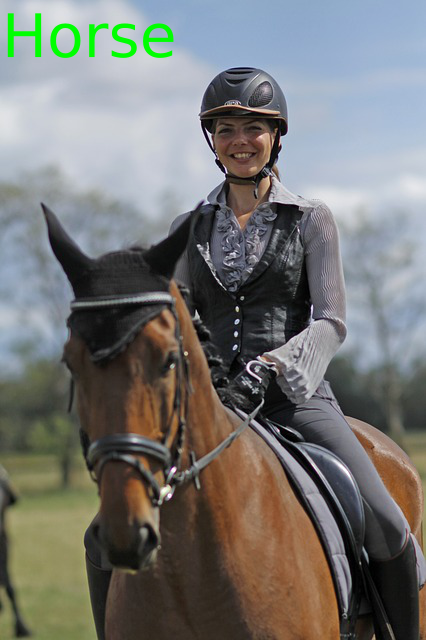
\includegraphics[width=\columnwidth]{figures/horsewoman_class.png}
        \caption{\textbf{Classification:} \\ The output is a one-dimensional label of the entire image. In this case the image can be classifed as showing a cat.}
        \label{fig:sfig1}
    \end{subfigure}\hspace{0.004\textwidth}
    \begin{subfigure}[t]{0.32\columnwidth}
        \centering
        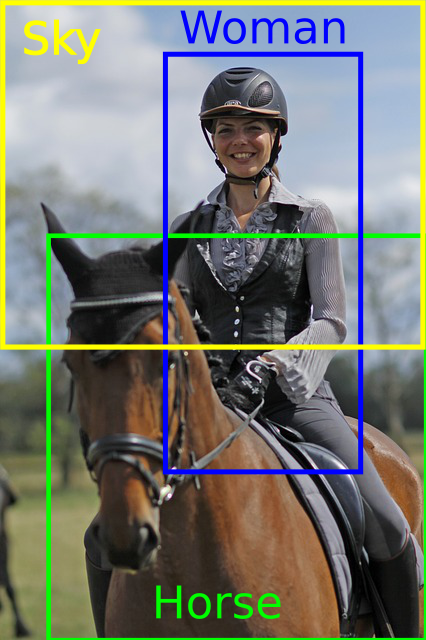
\includegraphics[width=\columnwidth]{figures/horsewoman_loc.png}
        \caption{ \textbf{Localization and Detection:}\\ The output are one or several bounding boxes together with a class label for each box.}
        \label{fig:sfig2}
    \end{subfigure} \hspace{0.004\textwidth}
    \begin{subfigure}[t]{0.32\columnwidth}
        \centering
        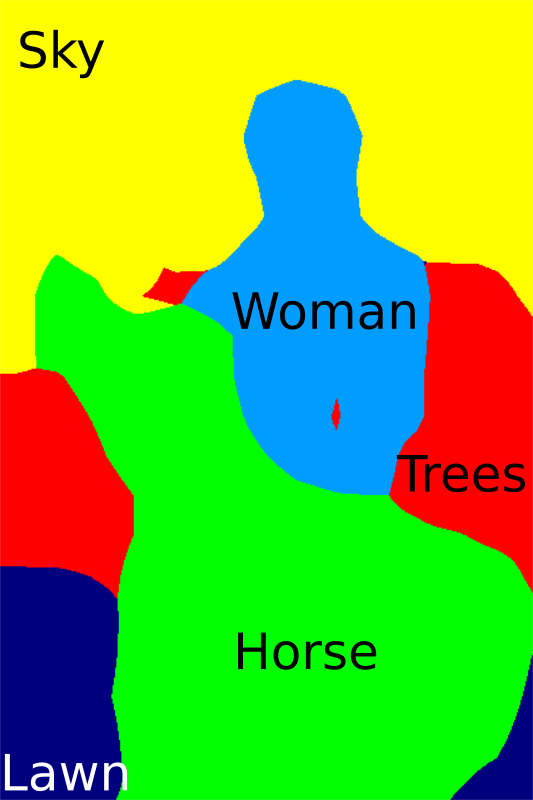
\includegraphics[width=\columnwidth]{figures/horse_seg.png}
        \caption{ \textbf{Segmentation:} \\
		The output is a class label for each pixel. The task is hence to regognize objects on a pixel-level.}
        \label{fig:sfig3}
    \end{subfigure}
    \caption{A visual comparision of computer vision task. The input in all three cases is the same image. The expected output is drawn on top of the input image.}
    \label{fig:cvtasks}
\end{figure*}



Three very important Computer Vision Tasks are \emph{Classification}, \emph{Detection} and \emph{Semantic Segmentation}. In all three tasks the algorithms receive a single image as input. However the output differs. In \emph{classification} a one-dimensional label is expected, representing the contained of the entire image in a single nominal value. The classes are usually choosen such that these values can be interpreted by humans (i.e. image of a car). In \emph{Localization} and \emph{Detection} the output of the algorithm is a set of bounding boxes, each assigned with a class label. 

\subsection{Relation between Tasks}

\subsection{Datasets}


All of the three task have as input a single image, but differ in the expected output.


There is  a close 

TODO: Finish paragraph

\iffalse

\section{Historical Review}\label{sec:review}



Krizhevsky et. al \cite{AlexNet} won the .

AlexNet was improved by several Authors in the succeeding years to achieve even better classification results in the ILSVRC-2013 and 2014. Most notable are GoogLeNet \cite{googLeNeT} and VGG16 \cite{VGG16}. Being designed independently, both Networks utilize filters with very small kernel size ($3\times 3$ and $1 \times 1$) and other parameter reduction techniques in order to severely increase the depths of their network.


\cite{AlexNet} al introduced a novel \gls{CNN} architecture. 

\fi







